\section{Labeling eigenvalues according to Briggs' criterion}\label{app:Briggs}

To evaluate $\mathcal{J}(\cdot)$ and $\mathcal{J}^{(R)}(\cdot)$, we must know whether an eigenvalue is upstream- or downstream-going, which we can do using Briggs' criterion (see definition~\ref{def:Briggs}). By proposition~\ref{prop:Briggs}, $M(s)$ has $N_+$ downstream- and $N_-$ upstream-going eigenvalues so that taking $\eta\to\infty$ yields $N_+$ eigenvalues with $\mathcal{I}(\alpha)>0$ and $N_-$ eigenvalues with $\mathcal{I}(\alpha)<0$. In principle, we can choose a large value of $\eta$ such that there $N_+$ eigenvalues with $\mathcal{I}(\alpha)>0$ and $N_-$ eigenvalues with $\mathcal{I}(\alpha)<0$, and then slowly decrease $\eta$ to zero while tracking the eigenvalues (since they are a continuous function of $\eta$) to assign a label of upstream- or downstream-going. However, for problems of interest, the sign of $\mathcal{I}(\alpha)$ remains the same for most eigenvalues as $\eta$ increases, as shown in figure~\ref{fig:Bertolotti_Briggs_main}. For this configuration, the sign of $\mathcal{I}(\alpha)$ changes for only one eigenvalue, as shown in figure~\ref{fig:Bertolotti_Briggs_zoom}. Since the sign of $\mathcal{I}(\alpha)$ does not change as $\eta$ increases for most eigenvalues, we choose the smallest $\eta>0$ such that there $N_+$ eigenvalues with $\mathcal{I}(\alpha)>0$ and call it $\eta_{\mathrm{opt}}$ (see algorithm~\ref{alg:briggsSub}). Then we match each eigenvalue associated with $\eta_{\mathrm{opt}}$ to the closest eigenvalue associated with $\eta=0$, where we measure distance as $|\alpha(\eta_{\mathrm{opt}}-i\omega)-\alpha(-i\omega)|$ (see algorithm~\ref{alg:briggs}). There is no guarantee that this algorithm will always correctly label the eigenvalues, but we have found this to work well in-practice. Moreover, if an eigenvalue is labeled incorrectly, then the OWNS march will not be well-posed and will fail. Therefore, any failure in labeling the eigenvalues will be easy to identify.

\begin{figure}
    \centering
    \begin{subfigure}[b]{0.48\textwidth}
        \centering
        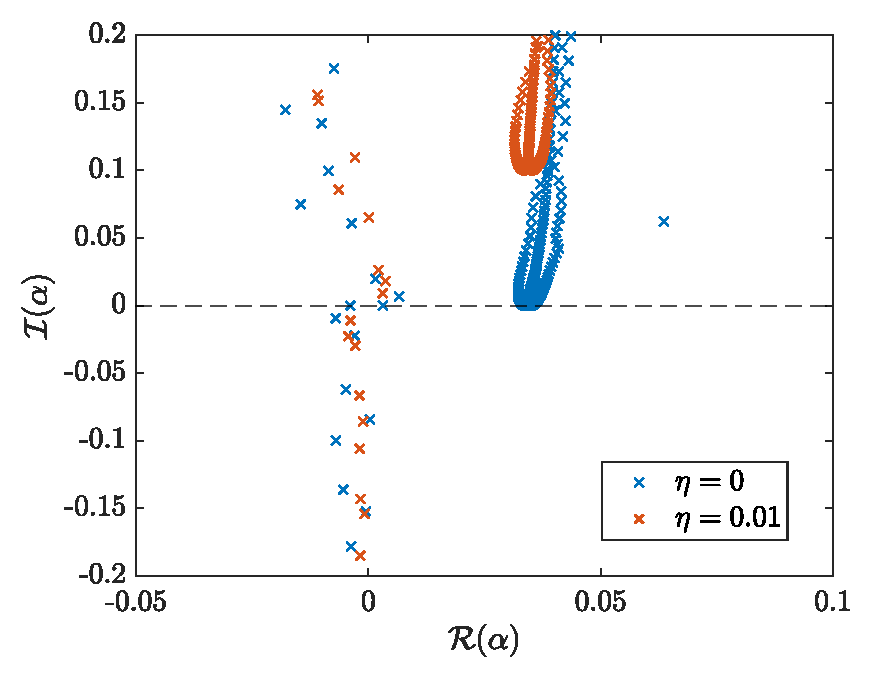
\includegraphics[width=1\linewidth]{figures/Bertolotti_Briggs.pdf}
        \caption{}\label{fig:Bertolotti_Briggs_main}
        \end{subfigure}
    \begin{subfigure}[b]{0.48\textwidth}
        \centering
        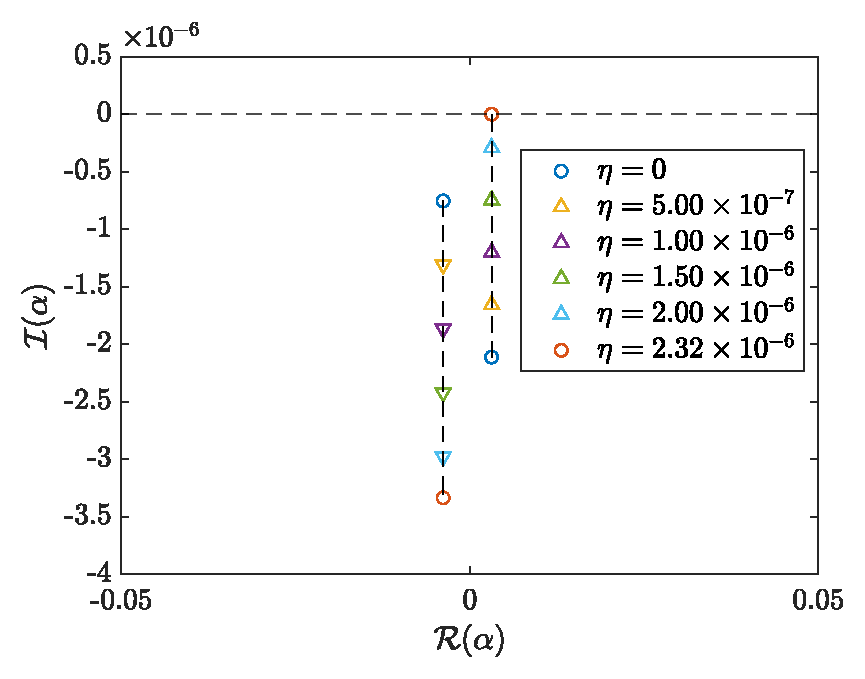
\includegraphics[width=1\linewidth]{figures/Bertolotti_Briggs_1.pdf}
        \caption{}
        \label{fig:Bertolotti_Briggs_zoom}
    \end{subfigure}
    \caption{Spectrum of TS wave at $\mathrm{Re}_x=1.6\times10^5$ for different values of $\eta$.}
    \label{fig:Bertolotti_Briggs}
\end{figure}


\begin{algorithm}
\caption{Bisection search for smallest $\eta$ such that there are $N_+$ eigenvalues with $\mathcal{I}(\alpha)>0$ and $N_-$ eigenvalues with $\mathcal{I}(\alpha)<0$}\label{alg:briggsSub}
\begin{algorithmic}
\State\textbf{Input}: (real) frequency $\omega$
\State $\eta_{\max} \gets 1$, $\eta_{\min} \gets 0$
\While{$\eta_{\max}-\eta_{\min} > \eta_{\max}\times 10^{-3}$}
\State $\eta\gets (\eta_{\min}+\eta_{\max})/2$
\State $\bm{\alpha} \gets$ eigenvalues of $M(\eta-i\omega)$
\State $\tilde{N}_+\gets$ number of $\alpha$ such that $\mathcal{I}(\alpha_i)>0$ for $i=1,\dots,N$
\State $\tilde{N}_-\gets$ number of $\alpha$ such that $\mathcal{I}(\alpha_i)<0$ for $i=1,\dots,N$
\If{$\tilde{N}_+=N_+$ and $\tilde{N}_-=N_-$}
\State $\eta_{\max}\gets\eta$
\Else
\State $\eta_{\min}\gets\eta$
\EndIf
\EndWhile
\State $\mathrm{eta}_{\mathrm{opt}}\gets\eta$
\State\textbf{return} $\eta_{\mathrm{opt}}$
\end{algorithmic}
\end{algorithm}

\begin{algorithm}
\caption{Apply Briggs' criterion to label eigenvalues}\label{alg:briggs}
\begin{algorithmic}
\State Given a (real) frequency $\omega$, compute $\eta_{\mathrm{opt}}$ using algorithm~\ref{alg:briggsSub}
\State $\bm{\alpha}_{\mathrm{opt}}\gets$ eigenvalues of $M(\eta_{\mathrm{opt}}-i\omega)$
\State $\bm{\alpha}_{\mathrm{zero}} \gets$ eigenvalues of $M(-i\omega)$
\State $\tilde{N}_+^{\mathrm{zero}}\gets$ number of $\alpha_{\mathrm{zero}}$ such that $\mathcal{I}(\alpha_{\mathrm{zero},i})>0$ for $i=1,\dots,N$
\State $\tilde{N}_-^{\mathrm{zero}}\gets$ number of $\alpha_{\mathrm{zero}}$ such that $\mathcal{I}(\alpha_{\mathrm{zero},i})<0$ for $i=1,\dots,N$
\State $\tilde{N}_+^{\mathrm{opt}}\gets$ number of $\alpha_{\mathrm{opt}}$ such that $\mathcal{I}(\alpha_{\mathrm{opt},i})>0$ for $i=1,\dots,N$
\State $\tilde{N}_-^{\mathrm{opt}}\gets$ number of $\alpha_{\mathrm{opt}}$ such that $\mathcal{I}(\alpha_{\mathrm{opt},i})<0$ for $i=1,\dots,N$
\State $N_{\mathrm{flip}}\gets|\tilde{N}_+^{\mathrm{zero}}-\tilde{N}_+^{\mathrm{opt}}|$
\State $N_{\mathrm{count}} \gets 0$, $i\gets0$, $\bm{\alpha}_+\gets \{\}$, $\bm{\alpha}_-\gets \{\}$
\While{$N_{\mathrm{count}} < N_{\mathrm{flip}}$}
\State $i\gets i + 1$
\State $j\gets\arg\min_{j=1,\dots,N}|\alpha_{\mathrm{zero},i}-\alpha_{\mathrm{opt},j}|$.
\If{$\mathrm{sign}(\mathcal{I}(\alpha_{\mathrm{zero},i}))\neq\mathrm{sign}(\mathcal{I}(\alpha_{\mathrm{opt},j}))$}
\State $N_{\mathrm{count}}\gets N_{\mathrm{count}} + 1$
\If{$\mathrm{sign}(\mathcal{I}(\alpha_{\mathrm{zero},i}))>0$}
\State $\bm{\alpha}_-\gets$ append $\alpha_{\mathrm{zero},i}$
\Else
\State $\bm{\alpha}_+\gets$ append $\alpha_{\mathrm{zero},i}$
\EndIf
\Else
\If{$\mathrm{sign}(\mathcal{I}(\alpha_{\mathrm{zero},i}))>0$}
\State $\bm{\alpha}_+\gets$ append $\alpha_{\mathrm{zero},i}$
\Else
\State $\bm{\alpha}_-\gets$ append $\alpha_{\mathrm{zero},i}$
\EndIf
\EndIf
\EndWhile
\end{algorithmic}
\end{algorithm}